% 张量扰动
对于在视界内部的模式来说,张量扰动对应了在FRW背景下传播的引力波.

\subsection{宇宙演化}
在共形牛顿规范下,我们只保留$h_{ij}^{TT}$,可得
\begin{equation}
ds^2 = a^2[-d  \eta^2+(\delta_{ij}+h_{ij}^{TT})dx^i dx^j ]~.
\end{equation}
对于爱因斯坦张量,我们有$\delta G^0_0 = 0, \delta G^i_0 = 0$以及
\begin{equation}
\delta G^i_j = \frac{1}{2 a^2} [ (h_{ij}^{TT}  )'' + 2\mathcal H (h_{ij}^{TT})' - \nabla^2 h_{ij}^{TT}  ]~.
\end{equation}
于是,扰动的爱因斯坦方程可以写成如下形式
\begin{equation}\label{TenPT_eq1}
(h_{ij}^{TT})'' + 2 \mathcal H (h_{ij}^{TT})' - \nabla^2 h_{ij}^{TT} = 16 \pi G a^2 \sigma_{ij}^{TT} ~.
\end{equation}
我们可以换到动量空间然后以极化张量为基进行如下展开
\begin{equation}
\tilde h_{ij}^{TT} (\eta,\mathbf k) = \sum_{A = +,\times} e^A_{ij} (\hat{\mathbf k}) \tilde h_A (\eta,\mathbf k)~, 
\end{equation}
类似地,我们有
\begin{equation}
\tilde \sigma_{ij}^{TT} (\eta,\mathbf k) = \sum_{A = +,\times} e^A_{ij} (\hat{\mathbf k}) \tilde \sigma_A (\eta,\mathbf k) ~.
\end{equation}
极化张量的定义如下
\begin{equation}
\begin{aligned}
e^+_{ij}(\hat{\mathbf k}) & = \hat{\mathbf u}_i \hat{\mathbf u}_j - \hat{\mathbf v}_i \hat{\mathbf v}_j ~, \\
e^\times_{ij} (\hat{\mathbf k}) & = \hat{\mathbf u}_i 
\hat{\mathbf v}_j + \hat{\mathbf v}_i \hat{\mathbf u}_j~,
\end{aligned}
\end{equation}
极化张量按照下式归一化
\begin{equation}
e^A_{ij} (\hat{\mathbf k}) e^{A'}_{ij} (\hat{\mathbf k}) = 2 \delta^{AA'} ~.
\end{equation}
如果$\hat{\mathbf k}$是沿着$\hat z$方向的,我们可以选取$\hat{\mathbf u} = \hat{\mathbf x}$以及$\hat{\mathbf v} = \hat{\mathbf y}$于是我们有
\begin{equation}
e^+_{ab} = \begin{pmatrix}
1 & 0 \\
0 & -1 
\end{pmatrix} \quad 
e^\times_{ab} = \begin{pmatrix}
0 & 1 \\
1 & 0
\end{pmatrix}
~.
\end{equation}
于是\autoref{TenPT_eq1} 变成了两个关于$h_A(\eta,k)$的独立方程
\begin{equation}\label{TenPT_eq2}
\tilde h''_A + 2 \mathcal H \tilde h'_A + k^2\tilde h_A = 16 \pi G a^2 \tilde \sigma_A ~.
\end{equation}
因此
\begin{equation}
\tilde h_A(\eta,\mathbf k) \propto \frac{1}{a(\eta)} \sin(k\eta+\alpha)  \quad (k\eta \ll 1) ~.
\end{equation}
假如
\begin{equation}
h_A(\eta,\mathbf k) \propto \frac{1}{a(\eta)} \sin(k\eta+\alpha)   ~.
\end{equation}
我们就有
\begin{equation}
h'_A(\eta,\mathbf k) \propto \frac{k \cos(k\eta+\alpha)}{a(\eta)} + O \bigg( \frac{1}{a^2} \bigg) ~,
\end{equation}
于是
\begin{equation}
\dot h_A (\eta,\mathbf k) \propto \frac{k\cos(k\eta+\alpha)}{a^2 (\eta)} + O \bigg( \frac{1}{a^3} \bigg)~.
\end{equation}
因为引力波的强度正比于$\sum_A\langle \dot h_A^2 \rangle$. 所以我们得出了$\rho_{\rm gw} \propto a^{-4}$. 需要注意的是,只有张量在视界内的时候,它们才能够被引力子描述,也就是一些能量和动量都是能被很好定义的,随着宇宙的膨胀,能量密度按照$1/a^4$变化.

对于超出视界的模式,我们有
\begin{equation}
\tilde h'' + \frac{2}{\eta} \tilde h' \simeq 0 ~,
\end{equation}
我们把初始条件$\eta_{\rm in}$设在辐射为主导的时期,初始条件设成$\tilde h(\eta_{\rm in},k) = \tilde h_{\rm in} (k)$以及$\tilde h'(\eta_{\rm in},k) = 0$. 由于\autoref{TenPT_eq2} 是一个线性方程,不同动量的模式不会混合.所以研究一个特定的模式如何演化我们可以简单地设置$\tilde h_{\rm in}(k) = 1$,也就是说,我们研究初始值为1下$\tilde h({\eta,k})$的演化.

为了方便数值积分,我们定义无量纲量$x = {\rm log} a$以及$\hat k = k/\mathcal H$于是运动方程变为了如下形式
\begin{equation}
\partial^2_x \tilde h + (3+\xi) \partial_x \tilde h + \hat k^2 \tilde h = 0 ~,
\end{equation}
\begin{figure}[ht]
\centering
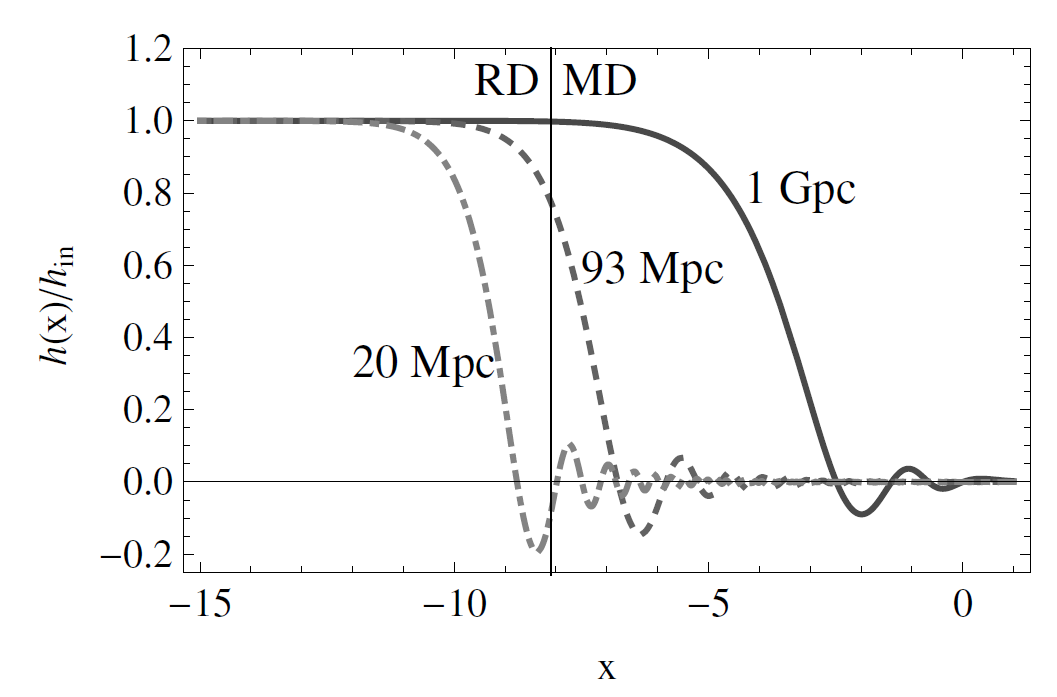
\includegraphics[width=14cm]{./figures/TenPT_1.png}
\caption{$\tilde h(\eta,k)$的演化.我们把初始条件设为1.横坐标是$x = {\log} \, a (\eta).$} \label{TenPT_fig1}
\end{figure}
我们在模拟中使用了这样的参数$\Omega_{\rm M}=0.3$以及$\Omega_{\Lambda} = 1 - \Omega_{\rm M} - \Omega_{\rm R} \simeq 0.7$. 数值模拟结果如\autoref{TenPT_fig1} 所示.

$\tilde h(\eta,k)$在视界外($k\eta\ll 1$)总是守恒的.进入世界之后,不管是在物质为主导时期还是辐射为主导的时期,它都会迅速衰变成0.到了退耦和时期,也就是红移$z_{\rm dec} \simeq 1090$, $x_{\rm dec}\simeq -7.0$, 所有的短波长引力波几乎都消失了,只有长波长的引力波仍然存在. 因此,引力波能影响大尺度上的微波背景辐射而影响不到小尺度上的微波背景辐射.

\subsection{辐射为主的时期的解析解}
辐射为主的时期的引力波运动方程为
\begin{equation}
\tilde h'' + \frac{2}{\eta} \tilde h' + k^2 \tilde h = 0~,
\end{equation}
这个方程有两个解$\sin(k\eta)/(k\eta)$和$\cos(k\eta)/(k\eta)$.加上边界条件$\tilde h(\eta_{\rm in},k) = \tilde h_{\rm in} (k)$以及$\tilde h'(\eta_{\rm in},k) = 0$. 边界条件确定了只有第一个解是可行的,所以我们有
\begin{equation}
\tilde h (\eta, k) \simeq \tilde h_{\rm in} \frac{\sin(k\eta)}{k\eta} ~.
\end{equation}

\subsection{物质为主的时期的解析解}
在物质为主的时期,我们有$\mathcal H = 2/\eta$,运动方程为
\begin{equation}
\tilde h'' + \frac{4}{\eta} \tilde h' + k^2 \tilde h = 0~.
\end{equation}
这个方程可以严格解,两个独立的解是
\begin{equation}
\begin{aligned}
h_1(\eta,k) & = \frac{1}{(k\eta)^2} \bigg[ \frac{\sin(k\eta)}{k\eta}  - \cos(k\eta) \bigg]~, \\
h_2(\eta,k) & = \frac{1}{(k\eta)^2} \bigg[ \frac{\cos(k\eta)}{k\eta} + \sin(k\eta) \bigg]~.
\end{aligned}
\end{equation}
我们考虑一个在物质-辐射平衡时期在视界外的模式,即$k\eta_{\rm eq}\ll 1$,在辐射为主的时期应为常数解.因为$h_1(\eta)$满足$h_1(0) = 1/3$以及$h'(0) = 0$,我们得到,在物质为主时期的长波长模式大约是下式
\begin{equation}
\tilde h (\eta,k) \simeq \frac{3\tilde h_{\rm in}(k)}{(k\tau)^2} \bigg[ \frac{\sin(k\eta)}{k\eta} - \cos(k\eta) \bigg], \quad k\eta_{\rm eq}\ll 1~.
\end{equation}


\subsection{宇宙学常数为主的时期的解析解}
宇宙学常数为主的时期,$\tilde h$满足的运动方程为
\begin{equation}
\tilde h'' - \frac{2}{\eta} \tilde h' + k^2 \tilde h = 0~.
\end{equation}
最一般的解为
\begin{equation}
\begin{aligned}
\tilde h(\eta,k) = \tilde h_{\rm in} \bigg\{ & \alpha_k [\cos(k\eta) + k\eta \sin(k\eta)] \\
+ & \beta_k [\sin(k\eta) - k\eta\cos(k\eta) ] \bigg\}~,
\end{aligned}
\end{equation}


















